
Previously, there was no tool for visualising and editing NeXus files. The screenshot below shows our solution for this and how we are implementing a tool containing this functionality. NeXus files are outputted by the experiment, and tools need to be configured to write them. This is currently being done manually by editing large JSON files which is both fragile and time-consuming.

\begin{figure}
\caption{Screenshot of the NeXus Constructor}
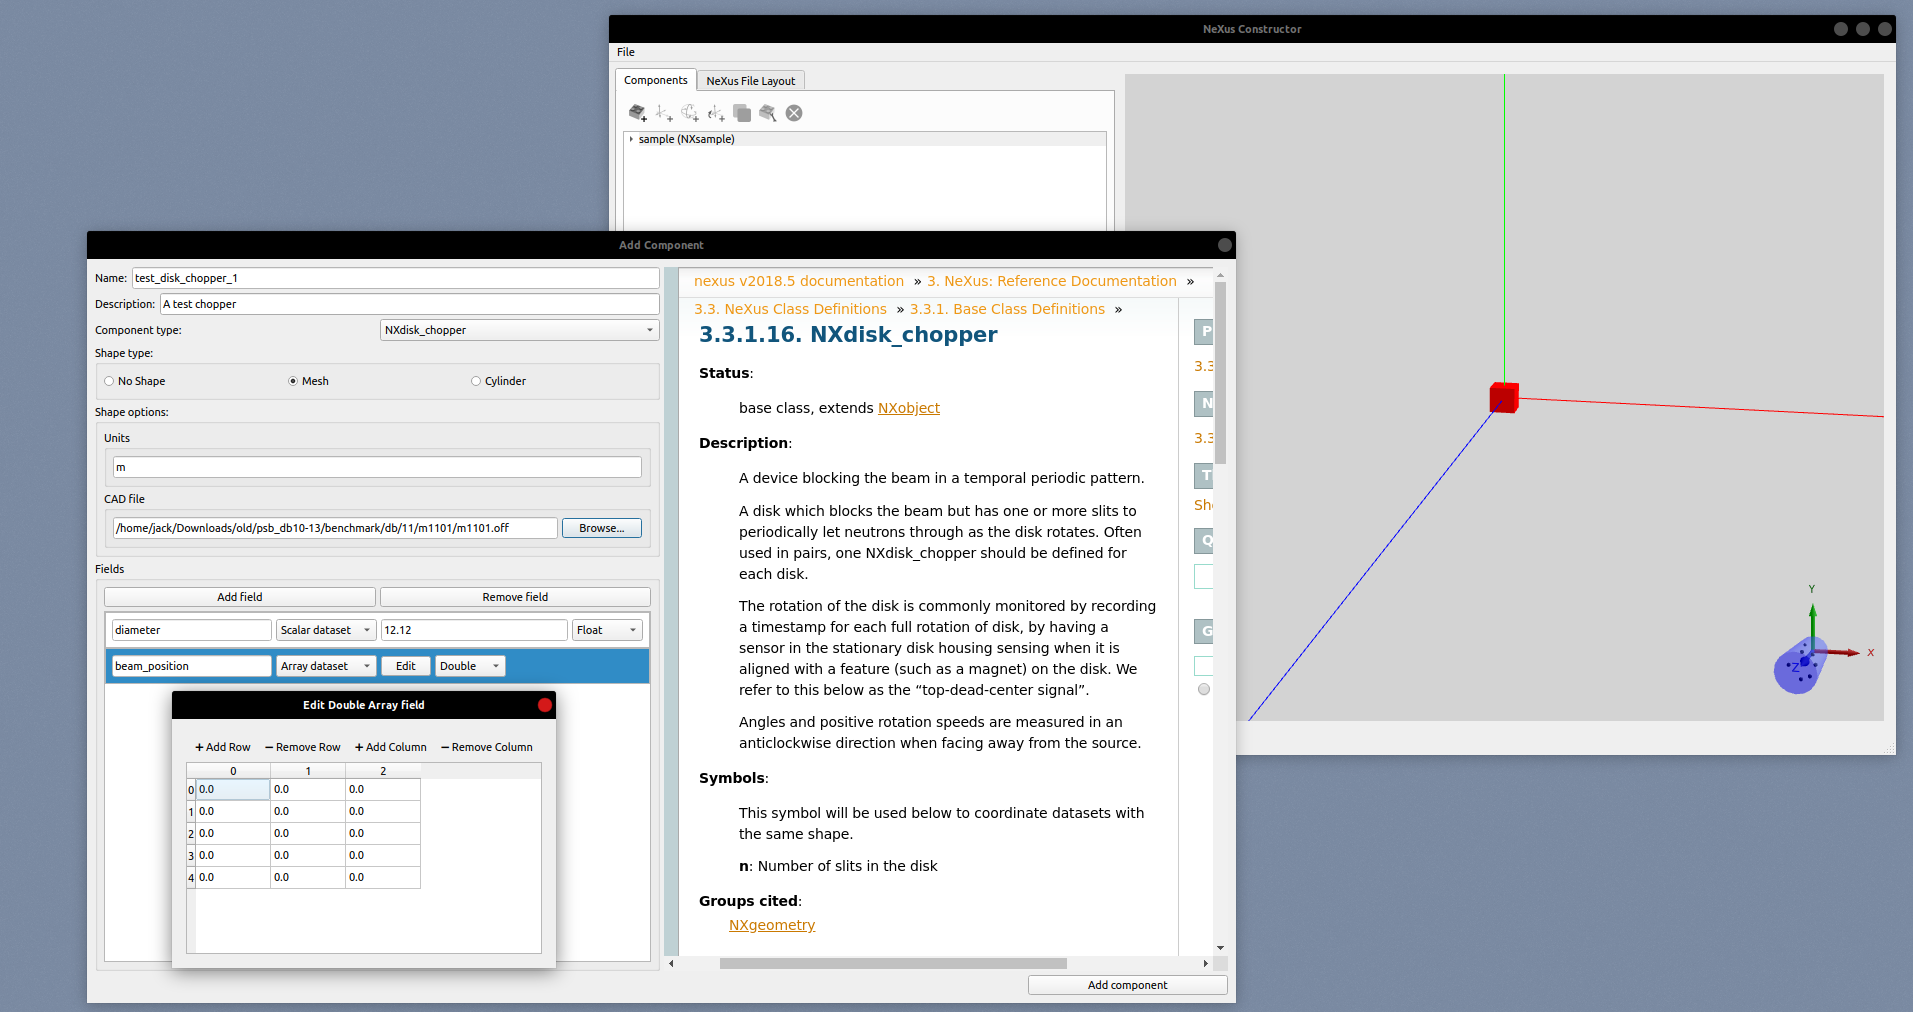
\includegraphics[width=\linewidth]{screenshot.png}
\end{figure}

The NeXus constructor is a tool written in Qt for Python which allows creating, editing and visualising NeXus files and their equivalent JSON files for configuring the experimental control software in order to write real-time data. 
